\documentclass[aps,twocolumn,preprintnumbers]{revtex4}

%The following packages add LaTeX commands that make formatting and writing math easier

\usepackage{graphicx}  % Include figure files
\usepackage{subfigure}

\linespread{1.1}
\usepackage{fancyhdr}
\usepackage{parskip}
\usepackage[T1]{fontenc}
\usepackage{dcolumn}   % Align table columns on decimal point

\usepackage{bm}        % bold math
\usepackage{amsfonts}  % Common math fonts
\usepackage{amsmath}   % Common math functions
\usepackage{amssymb}   % Common math symbols
\usepackage{gensymb}

\setlength{\parindent}{10pt}

%Custom commands for ease
\newcommand{\mm}{\mathrm{mm}}
\newcommand{\CPM}{\mathrm{CPM}}
\newcommand{\Joule}{\mathrm{J}}
\newcommand{\Celcius}{\degree \mathrm{C}}
\newcommand{\Kelvin}{\mathrm{K}}


\begin{document}

\title{Using Noise to Determining Thermodynamic Constants Test 1}

\author{Connor Lindsay}

\affiliation {\it Physics Department, University of California, Santa Barbara, CA 93106}

\date{July 2023}

\begin{abstract}
    Johnson noise in resistors relate the noise in voltages produced by itself to the Boltzmann constant the absolute temperature. In this paper we measured this noise in many resistors to determine these constants experimentally. From the we obtained that absolute zero is $-280 \pm 50 \Celcius $ and Boltzmann's constant is $(4.5 \pm 0.8)\times 10^{-23} \Joule/\Kelvin$. Absolute zero is defined as $-273.15 \Celcius$ which is mutually consistent with our results, while Boltzmann's constant is defined as $(4.5 \pm 0.8)\times 10^{-23} \Joule/\Kelvin$ which is 4 standard deviations away from our results. 
\end{abstract}

\maketitle


\section{Introduction}

When dealing with physics, often times there are constant inherent to our universe that pop up in theories. In thermodynamics two of the most important quantities are the Boltzmann constant, and the temperature of absolute zero. These are essential quantities for use in measurements, and so it is necessary to know them to high precision. Here I have focused on finding these through the phenomena of Johnson noise of Resistance electrical circuits.  

Johnson noise is a type of electrical noise that is due to the thermal motion of electrons within an electrical media. This is a result of electrons randomly moving within the object, causing small currents to flow along it, and thus voltages across the resistor. This noise is proportional to both the temperature and the temperature of the resistor and the resistance of itself. This noise also naturally frequency dependant, as everything has parasitic capacitance that couples to ground creating a low pass filter on the noise.

\begin{align}
     dV_f^2 &= 4R_f k_b T df
     \\
     R_f &= \frac{R}{1 + (2 \pi C R f)^2}
\end{align}

Here we use $R$ to be the DC resistance of the resistor, $C$ the DC capacitance of the resistor, $k_B$ as Boltzmann's constant, $T$ as absolute temperature, $f$ as frequency, and $d_f^2$ as the differential squared voltage at a given frequency produced by the noise. 

In order for this to be useful though this needs to go through heavy amplification as the voltage it outputs is very small. This naturally adds in another variable as the gain will not be constant across all voltages, so the voltage actually measured will be of a different form. 

\begin{equation}
    dV^2 = 4R k_B T \frac{g(f)^2 df}{1 + (2 \pi R C f)^2}
\end{equation}

So by measuring this Johnson noise it is then possible to calculate the absolute zero, and the Boltzmann experimentally. 

\section{Methods}

For practical reasons it is not feasible to measure the voltage across all frequencies, there is unwanted pink noise inherent to electrical equipment that we do not want to pick up, as well as AC power supply and monitor noise picked up by mutual inductance's that would alter the data. So remedy this the voltage across a specific frequency band will be analyzed. For this experiment I have used an SR760 spectral analyzer, a band pass filter, and a low noise amplifier for data collection, as well as a white noise generator for calibration of the equipment's gain function and a multi-meter for measurement of the resistors DC resistance. The resistors themselves were attached BNC connected for use in the amplifier. 

All voltage measurements were taken through the spectral analyzer, but the resistance and capacitance had to be measured separately. Resistances were measured using a high precision digital multi-meter, while capacitance seen by the system was only estimated using the specifications of the machinery. 

Voltage measurements we taken through these equipment as shown in the figure \ref{fig:Experimental Setup} below. To being, the resistor was hooked into the input of the amplifier with again of $5 \times 10^4$ and band-pass filter from 3kHz to 10kHz. This was fed into another band-pass filter from 3kHz to 10kHz and the finally into the spectral analyzer where the band voltage in this range could be read off. Since noise was being measured, I averaged over 2000 samples at a time to get data points to get an average value for the noise produced. 

\begin{figure}[h]
    \centering
    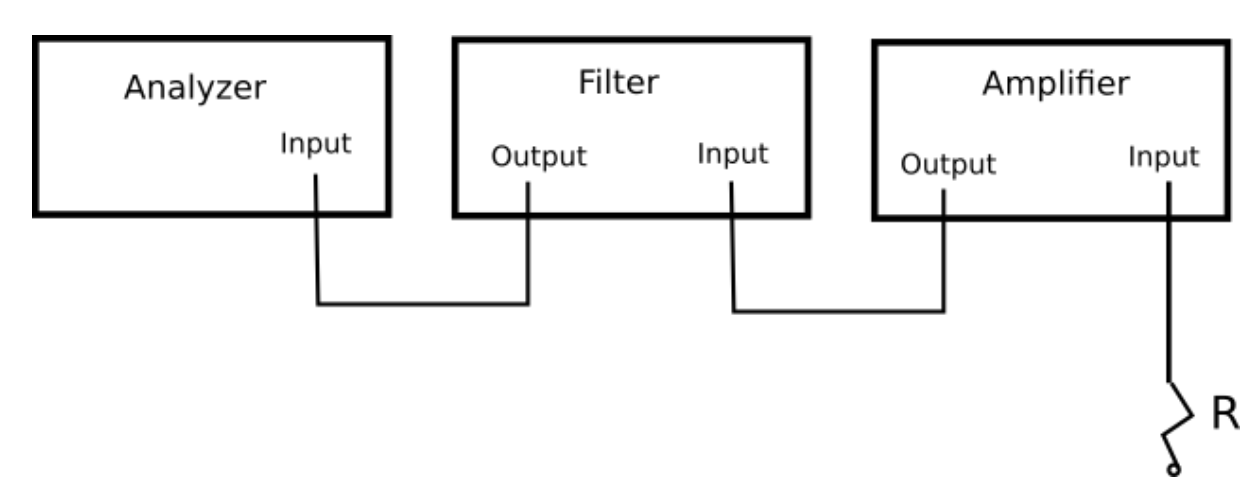
\includegraphics[width = 0.85\columnwidth]{Screenshot (16).png}
    \caption{Schematic of the setup for measuring Johnson Noise. The amplifier and filter get the noise to detectable levels within the 3kHz to 10kHz band that we care about, and the spectral analyzer then measures the voltage within this range.}
    \label{fig:Experimental Setup}
\end{figure}

20 points of data like this were collected from 6 different resistor as well as a shorted output. This shorted output gave the internal background rate, so we could extract the rate due to just the resistor attached to the output. 

\begin{equation}
    V_\mathrm{meas}^2 = V^2 + V_\mathrm{short}^2
\end{equation}

This was also collected at room temperature and while the resistors were cooled in liquid nitrogen, so that both the absolute zero and the Boltzmann constant could be calculated. The equation for Johnson noise gives the relation to these quantities when evaluated from 3kHz to 10kHz.  

\begin{equation}
    V^2 = 4 R k_B T \int^{10000}_{3000} \frac{g(f)^2 df}{1+ (2\pi RC f)^2}
\end{equation}

The only other matter is to calibrate the instruments by measuring the gain function. Measurement of the gain function was achieved by using the noise output from the white noise generator. To do this the output from the generator into the amplifier and filter was measured, and the output straight from the generator directly was measured. This was done 20 times both with the generator turned on and with the generator turned off. The generator was tuned so as to just barely not overload the amplifier, while on its maximum gain setting. This data was taken as 2000 sample sets of the voltage at each frequency over a range from 500Hz to 13000Hz so that the voltage directly from the generator could be extracted in a similar way to band analysis voltage before, and the the filtered voltage divided by the unfiltered voltage to get the gain at each frequency. 


\section{The Gain Function}

Most of the data processed in this experiment was to compute the gain function. The result of this can be seen in figure \ref{fig:Gain Function} where the data is plotted along with a polynomial fit. To gain function was computed from 4 sets data, measuring the voltage in decibel volts (dbV) at specific frequencies on the spectral analyzer. The data sets were computed for the filtered white noise $dbV_{fw}$, the filtered background noise $dbV_{fb}$, the direct or raw white noise $dbV_{rw}$ and the raw background noise $dbV_{rb}$. 20 measurements were taken for each of these sets, so the error in these was achieved by using the standard deviation for a sample from a population and dividing by $\sqrt{n}$ for $n$ samples. 

\begin{align}
    dbV &= \sum_i \frac{dbV_i}{n}
    \\
    \sigma_{dbV} &= \sqrt{ \frac{\sum_i (dbV - dbV_i)^2 }{n-1} }
\end{align}
Then we can convert these to voltages using the equation for decibels, and use those to get the voltages the true filtered ,$V_{ft} $, and raw voltages $V_{rt} $ without the background rate. 

\begin{align}
    V &= 10^{dbV/20} 
    \\
    \sigma_V &= \frac{\ln(10) V \sigma_{dbV}}{20}
    \\
    V_{t} &= \sqrt{V_{w}^2 - V_{b}^2 }
    \\
    \sigma_{V_t} &= \frac{\sqrt{V_w^2 \sigma_{V_w}^2 + V_r^2 \sigma_{V_r}^2} }{V_t}
\end{align}

Lastly the ratio of those two true voltages gives the gain of the system at that specific frequency. 

\begin{align}
    g = \frac{V_{ft}}{V_{rt}}
    \\
    \sigma_g = g \sqrt{ \frac{\sigma_{V_{ft}}^2}{V_{ft}^2} + \frac{\sigma_{V_{rt}}^2}{V_{rt}^2} }
\end{align}

The result of this calculation is shown in figure \ref{fig:Gain Function}, where it is plotted. A 10 term polynomial fit is also plotted against it so the general shape in the region between 3kHz and 10kHz can be seen. This fit fails at the tails of the data though so it is not very useful except for a general idea of the shape. 

\begin{figure}[h]
    \centering
    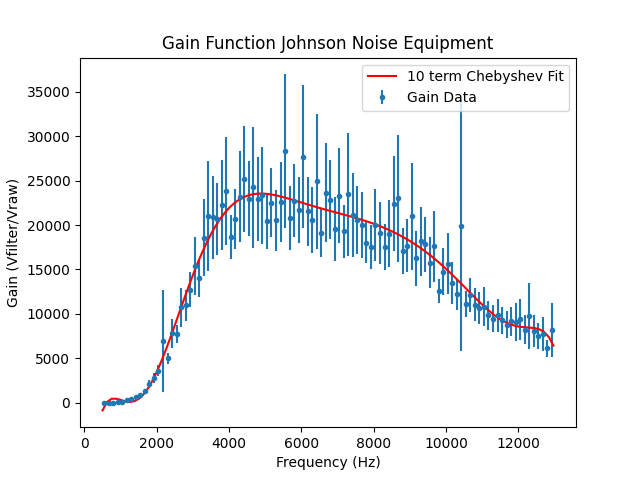
\includegraphics[width = 0.85\columnwidth]{GainFuction7-26.png}
    \caption{Using a white noise generator the system specific gain function can be measured. This is obtained by comparing the voltage output of the generator to itself after fed through the system, and the background noise of the system.}
    \label{fig:Gain Function}
\end{figure}

This then calibrates the system to the internal gain and its frequency dependence, so that only measurements of the resistors themselves need to be made after. For these specific measurements though the integral of the gain function must be taken. To do this trapezoidal approximation to the integral was used on the data points present. 

\begin{gather}
    \int_{3000}^{10000} \frac{g(f)^2 df}{1 + (2\pi RCf)^2} =
    \nonumber
    \\
    \sum_i \frac{1}{2} \bigg( \frac{g(f_i)^2 }{1 + (2\pi RCf_i)^2} + \frac{g(f_{i+1})^2 }{1 + (2\pi RCf_{i+1})^2} \bigg) \delta f_i 
\end{gather}

Here $i$ indexes each bin that the spectral analyzer output starting at 3kHz and going till 10kHz, and $\delta f_i$ is the difference between the frequency of adjacent bins. 

To get the uncertainty on this the partial derivatives with respect to each $g(f_i)$ as well as $R$ and $C$ were taken, and then these times their uncertainties in the respective quantities were summed in quadrature. The uncertainty in the frequency was negligible compared the uncertainty of the gain function itself so that was ignored. 



\section{Results}

Then with the gain function found, the band voltage can then be found from the resistors through the spectral analyzer, and then manipulated as in the above equations. 20 pieces of 2000 sample averaged data we taken for each resistor, and the usual average and standard deviation was obtained for each of them, after converting from dbV to V. This is in much the same procedure that was taken for the data obtained for the gain function, as in equations (6) through (11). Instead of finding a gain funtion afterwards though, the true voltage was squared in order to be used as in equation (5). Let us call $G$ the gain constant, a specific value of the total gain in that band based on the resistor itself and the gain function. 

\begin{equation}
    G = \int_{3000}^{10000} \frac{g(f)^2 df}{1 + (2\pi RCf)^2}
\end{equation}

We can then rearrange the equation to get it into a linear form so that the quantities of interest give the slope, that we can plot to fit as seen in figures \ref{fig:Room Temp} and \ref{fig:Liquid Nitrogen Fit}. The uncertainty in combined values is then calculated using the partial derivative rule added in quadrature.

\begin{align}
    \frac{V^2}{4G} &= (k_B T) R
    \\
    \sigma_{V^2/4G} &= \frac{V^2}{4G} \sqrt{\frac{4\sigma_{V}^2}{V^2} + \frac{\sigma_{G}^2}{16G^2}}
\end{align}



\begin{figure}[!htb]
    \centering
    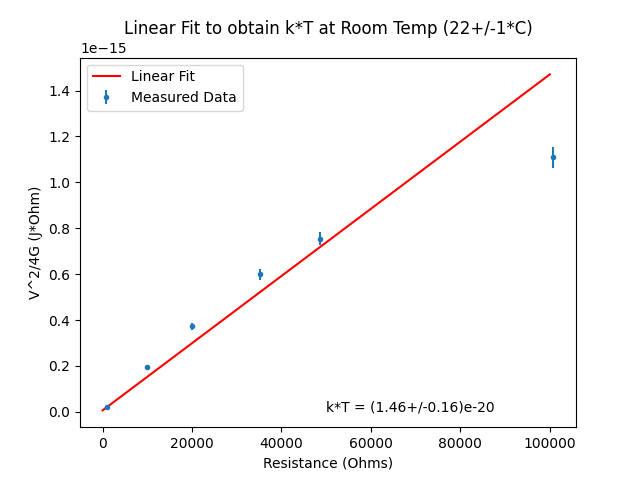
\includegraphics[width = 0.85\columnwidth]{RoomFit.png}
    \caption{By arranging the equations for Johnson noise, Boltzmann's constant and absolute temperature can be found as the slope of a linear plot. This particular data does not follow the predicted linear graph as a result of incorrect estimation of capacitance of the system.}
    \label{fig:Room Temp}
\end{figure}


\begin{figure}[!htb]
    \centering
    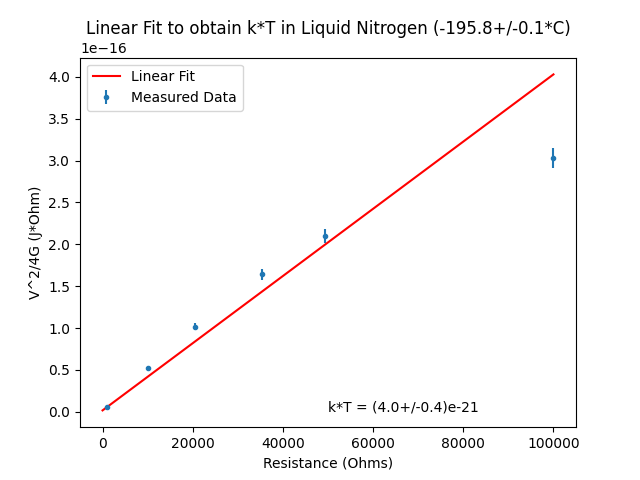
\includegraphics[width = 0.85\columnwidth]{LN2Fit.png}
    \caption{This again finds the Boltzmann constant and the absolute temperature as the slope of a graph. This follows the same curve as the graph at room temperature, showing that there was a large sytematic error present.}
    \label{fig:Liquid Nitrogen Fit}
\end{figure}

From these figures we can see that the value for $k_B T$ obtained at room temperature was $(1.46 \pm 0.16) \times 10^{-20} \Joule $ and at the temperature of liquid nitrogen we got $(4.0 \pm 0.4) \times 10^{-21} \Joule$. It is of particular note though that even though we expect these to adhere to a linear fit, the plotted points do not follow that path. This discrepancy is most likely caused by an error in the estimation for the capacitance in the gain function since there was no actual measurement done for that. By re-graphing with capacitance's an order of magnitude larger we get that this does follow a linear graph within the 1 standard deviation of the error bars.

This allows us to either solve for either the Boltzmann constant or absolute temperature using the accepted value of the other, or to solve for both at the same time. By using the known temperature of the resistor at the time of measurement in Celsius, we can relate that to the absolute temperature obtained to get what absolute zero in Celsius is. Letting the $K_R = (1.46 \pm 0.16) \times 10^{-20} \Joule$ our constant at room temperature, and $K_N = (4.0 \pm 0.4) \times 10^{-21} \Joule$ the same constant obtained at the temperature of liquid nitrogen, $C_R = 22\pm1 \Celcius$ the temperature of the room in Celcius, $C_N = -195.8 \pm 0.1 \Celcius$ the temperature of liquid nitrogen in Celsius, and $C_0$ absolute zero in Celsius we get the following equations. We also use the partial derivatives added in quadrature rule for calculating uncertainties. 

\begin{align}
    C_0 &= \frac{K_N C_R - K_R C_N}{K_R - K_N}
    \\
    k_B &= \frac{K_R - K_N}{C_R - C_N}
\end{align}

This gives a value of $-280 \pm 50 \Celcius $ for absolute zero in Celsius and $(4.5 \pm 0.8)\times 10^{-23} \Joule/\Kelvin$

Both of these have large margins of error, due mostly to the error of the slope fits themselves. If the data had been more linear as predicted, then the error margins would be significantly lower. 

The accepted value for absolute zero is $-273.15$ without any uncertainty since it is by definition. Our measurement agrees with this figure, but its uncertainty is very high so it is hard to tell how closely it agrees. The accepted value for Boltzmann's constant is $1.380649 \times 10^{-23} \Joule/\Kelvin$. This again is a defined quantity in the SI system and as such has no uncertainty. Our measurement does not agree with this value at all though. It is roughly 4 standard deviations, even with its large uncertainty, away from the experimentally obtained result, which indicates major flaws in the procedure. 

\begin{figure}[!htb]
    \centering
    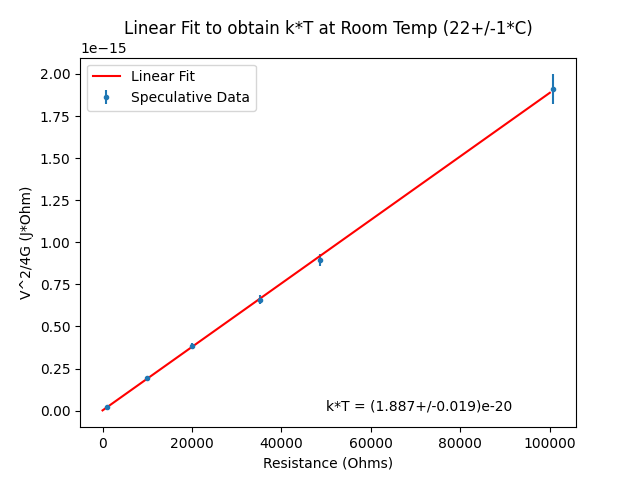
\includegraphics[width = 0.85\columnwidth]{RoomFitFix.png}
    \caption{Instead of the estimation of the capacitance of the system that relied on the specs of the equipment, I altered the capacitance using trial and error to minimize the uncertainty in the fit of the slope. The fit follows the linear shape closer because of this.}
    \label{fig:speculative data}
\end{figure}

The biggest flaw was in the estimation of the capacitance of the system as discussed above. Of all the values used this is the only one estimated instead of measured, and as such if we change our estimation we get much better results. Through trail and error it seems the system actually has a capacitance of $225 \pm 10 \mathrm{pF}$ instead of the original estimation of $20 \pm 1\mathrm{pF} $. As we can see in figure \ref{fig:speculative data} the data does follow the expected linear slope very well when using this capacitance. 

This gives an entire order of magnitude better uncertainty on the slope of this fit, as well as altering the value of the fit by over $50 \%$. A different method would need to be devised to find the capacitance of the system then, or possibly a away to measure it is necessary, so that the data better follows the predictions. 

\section{Discussion}

The results of this are both better and worse than was expected. When preparing the experiment two sources of error stood out. For one the estimation of the capacitance of the system seemed very arbitrary and as such it seemed as though it would hinder the accuracy of the final result, and as well the measurement of the gain function could have been done in better ways. 

As was shown in figure \ref{fig:speculative data}, the capacitance estimate was most likely very far off from the true capacitance of the system and that contributed to the ill fit of the data. Taking an actual measurement of the capacitance of the system would allow for much more confidence in the final result. In addition the error in the slope of the linear fit accounted for the largest portion of the error in the final results for Boltzmann's constant and absolute zero, so better fitting data would also improve the precision of the final result. 

As seen in figure \ref{fig:Gain Function}, the values obtained for this had quite large uncertainty, which was due to a poor method in data collection. I used the largest gain value on the amplifier, and adjusted the white noise to that, but that meant that the white noise was less than a decibel above the background noise value on average. This resulted in very poor signal to noise ratios on the white noise voltage level, which propagated through to the final gain function. Either taking much larger data sets for the unfiltered background and white noise voltages, or using a smaller gain on the amplifier so the white noise used could be higher would improve the uncertainty in the gain function. 

One other place of improvement could be taking data over many different temperatures. Instead of solving for these values based on the two temperatures used, it could instead be plotted linearly using the temperature in Celsius as the independent variable to get a fit for Boltzmann's constant and absolute zero. 

\end{document}
